% Title:    A LaTeX Template For Responses To a Referees' Reports
% Author:   Petr Zemek <s3rvac@gmail.com>
% Homepage: https://blog.petrzemek.net/2016/07/17/latex-template-for-responses-to-referees-reports/
% License:  CC BY 4.0 (https://creativecommons.org/licenses/by/4.0/)
\documentclass[10pt]{article}

% Allow Unicode input (alternatively, you can use XeLaTeX or LuaLaTeX)
\usepackage[utf8]{inputenc}
\usepackage{hyperref}
\usepackage{xcolor}
\usepackage{todonotes}

\usepackage{microtype,xparse,tcolorbox}
\newenvironment{reviewer-commentX}{}{}
\tcbuselibrary{skins}
\tcolorboxenvironment{reviewer-comment }{empty,
  left = 1em, top = 1ex, bottom = 1ex,
  borderline west = {2pt} {0pt} {black!20},
}
\ExplSyntaxOn
\NewDocumentEnvironment {response} { +m O{black!20} } {
  \IfValueT {#1} {
    \begin{reviewer-commentX}
      \setlength\parindent{2em}
      \noindent
      \ttfamily #1
    \end{reviewer-commentX}
  }
  \par\noindent\ignorespaces\color{blue}
} { \bigskip\par }

\NewDocumentCommand \Reviewer { m } {
  \section*{Comments~by~Reviewer~#1}
}

\NewDocumentCommand \Editor { m } {
  \section*{Comments~by~Editor}
}

\NewDocumentCommand \ToolComments { m } {
  \section*{Tool~Comments~by~Reviewer~#1}
}

\ExplSyntaxOff
\AtBeginDocument{\maketitle\thispagestyle{empty}\noindent}

% You can get probably get rid of these definitions:
\newcommand\meta[1]{$\langle\hbox{#1}\rangle$}
\newcommand\PaperTitle[1]{``\textit{#1}''}

\title{Response letter to EMISAJ Manuscript entitled "Multi-level modeling with Openflexo/FML- A contribution to the MULTI process challenge"}
%\author{Author1 \and Author2 \and Author3}
\date{\today}

\begin{document}

Dear Editor,

\bigskip
Thanks for your message of August 16th, 2021, in which you suggested preparing a revision of our manuscript  \textbf{Multi-level modeling with Openflexo/FML- A contribution to the MULTI process challenge}.

\bigskip
We are grateful to the reviewers for their interest, effort, and suggestions. The  following pages detail how we have addressed the reviewers' concerns. We are confident that the paper is now improved, and hope that you will agree. The responses to the comments are organized on a per-reviewer basis, focusing, as suggested, on:

\begin{itemize}
\item Improving the presentation.
\item Providing a more explicit description of how the multi-level modeling emulation is achieved.
\item Discussing the general advantages and limitations of the multi-level emulation, including a clarification of what the implications would be of supporting more "levels" than the challenge required.
\end{itemize}

Moreover, the paper has been thoroughly revised to fix minor issues and to give the additional clarifications required by the reviewers. Please let us know if you need any further information or clarification.

\bigskip
Sincerely yours,

\bigskip
Sylvain, Joël, Jean-Christophe, Antoine, Fabien and Salvador

\pagebreak

\Editor{}

\begin{response}{The reviewers have made suggestions for improving the presentation but also raised a number of issues requiring clarification. An overarching theme is the request for a more explicit description of how the multi-level modelling emulation is achieved and what its general advantages and limitations are, including a clarification of what the implications would be of supporting more "levels" than the challenge required.}
%We have been more explicit to explain how we use the FML language at the end of the introduction, and in various figures. TODO.

We have improved the presentation of both, Openflexo/FML and our solution to the challenge so that: 1) the techniques we use to \emph{achieve} multi-level capabilities are more explicit; and, 2) the advantages and disadvantages of using them in order to fulfill the challenge requirements become clearer. Notably, we have added many details in the final paragraphs of the introduction section, improved the Section 2, devoted to the description of Openflexo, refactored figures 2, 4, 5, 6, 7 and 9 and, added figures 3 and 10.
\end{response}


\begin{response}{We very much welcome a "conventional" response to the challenge but would like to see the respective reviewer questions addressed in a revised version which is explicit as possible about the advantages and the disadvantages of the emulation. You may find the references listed below useful to keep explanations concise by referencing related work (note that reviewer 3's "Type-Instance pattern" is also known as the "Type Object" pattern). You should also respond to other concerns reviewers raise, either by making changes to the submission or in the form of an authors' response.}

%\textcolor{orange}{
In the answer to the previous editor's comment, we describe the improvements of our revision, which includes an emphasis in discussing trade-offs related to the emulation of multi-level modeling by using the Openflexo/FML and the type-object pattern. Additionally, the related work section has been extended in order to enhance the comparison between our approach and previous solutions to the challenge.%}
% fd ok
% sg ok
% jc ok

%\todo[inline]{I do not understand this answer. We are saying that other approaches are also unconventional?}
\end{response}


\begin{response}{Finally, to achieve consistency with other submissions, could you please change the subtitle to "A Contribution to the Multi-Level Process Challenge"?}

Done.
\end{response}

\pagebreak

\Reviewer{\#1}
\begin{response}{In section 2 Technology the authors describe the foundations of the Openflexo approach. Here it would greatly help the reader to see an example how the approach works for traditional modeling languages. For example, how would you realize a small subset of BPMN with the approach? This could briefly be illustrated so as to give the reader an immediate understanding. Especially, the 'metamodel'-agnostic approach seems very interesting but I would like to see how that is used for traditional modeling approaches.}

The Figure \ref{fig:BPMNSubsetExample} (above) shows how to realize a small subset of BPMN with Openflexo/FML (assuming a metamodel of the full specification of BPMN exists). Concretely, we show  how a virtual model (\texttt{SimplifiedBPMN}) can filter an existing model (BPMN) and be instantiated. Note that connection with external sources is not required for our solution to the challenge and is only represented in order to illustrate the capabilities of Openflexo/FML. Therefore, in the article we choose not to give this level of detail and focus on the left part of the figure.
% Fabien OK pour moi
% sg ok
% jc ok


\begin{figure}[t]
    \centering
    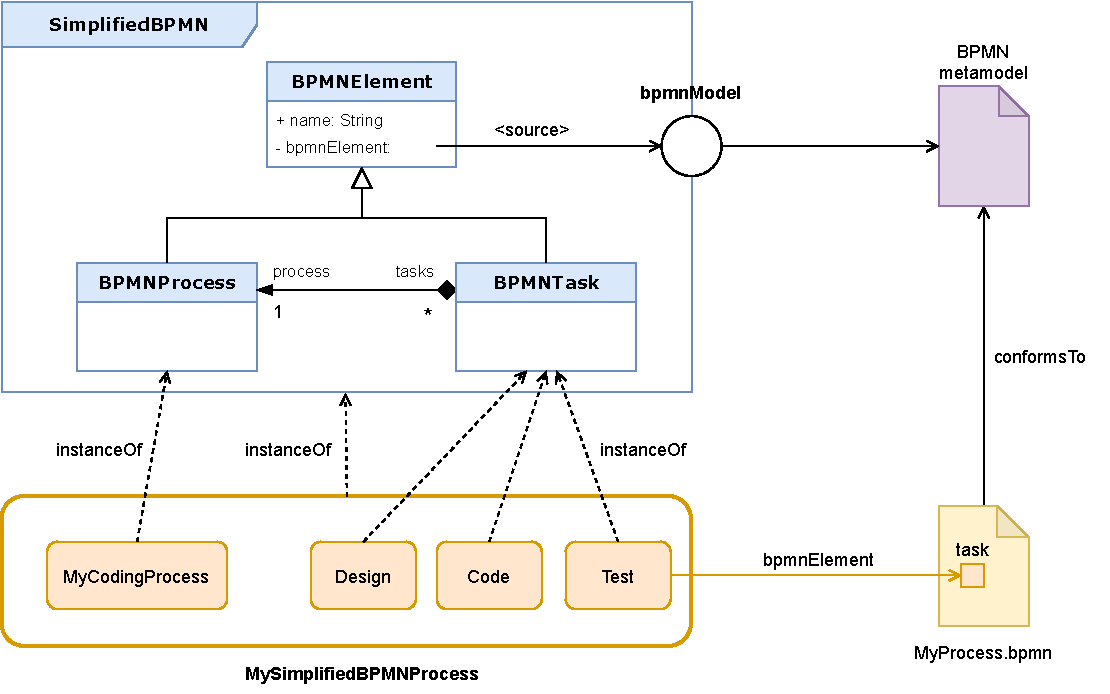
\includegraphics[width=1.0 \textwidth]{Figures/BPMNSubsetExampleWithExternalConnexion.pdf}
    \caption{An example of BPMN subset built on top of a BPMN/EMF model}
    \label{fig:BPMNSubsetExample}
\end{figure}

%non (jc)
%\todo{SG: Est ce possible de rajouter ce listing ou ca n'avance à rien ?. SM: If you want to add it, it should be ok, but remember then to update the answer text.}

%\begin{lstlisting}
%use org.openflexo.technologyadapter.emf.EMFModelSlot as EMF;
%import ["http://www.omg.org/spec/BPMN/20100524/MODEL-XMI"] as BPMN_METAMODEL;
%
%// A simplified BPMN metamodel exposing
%// both concepts BPMNProcess and BPMNTask
%model SimplifiedBPMN {
%
%  // Connexion to a .bpmn file
%  EMFModel bpmnModel
%    with EMF::EMFModelSlot(
%        metaModel = BPMN_METAMODEL);
%
%  // Abstract concept BPMNElement defining
%  // a name and a link to an eventual BPMNElement
%  // in .bpmn file
%  abstract concept BPMNElement {
%  	EMFObjectIndividual bpmnElement
%  	    with EMF::EMFObjectIndividualRole (
%			source = bpmnModel
%		);
%    String name values bpmnElement.name;
%  }
%
%  concept BPMNProcess extends BPMNElement {
%
%    // Describe here properties and
%    // behaviours for BPMNProcess concept
%    ...
%
%    concept BPMNTask extends BPMNElement {
%
%        // Describe here properties and
%        // behaviours for BPMNTask concept
%        ...
%
%    }
%
%    // Other core concepts
%  }
%}
%\textbf{}\end{lstlisting}

\end{response}

\begin{response}{Also, at the stage of section 2, the characterization of the FML language should be made clearer. The metamodel in Figure 2 seems mainly conceptual - but at the same time you refer to it as a basis for implementation. Could that be clarified? eg you have the class "Behavior" - which is a concept and I did not understand right away what it is composed of. On the other hand you have for example the class "ModelSlot" which seems like a very technical realization. Also, you note that roles have types but I could not find any types in the metamodel (?). Thus, I propose to include a more detailed version of your metamodel at this stage. Please note that EMISAJ does not have a page limitation, so no worries if that should require more space.}

%\textcolor{orange}{
We agree with the reviewer. The previous version of the figure depicting the main concepts of the FML language (Figure 2) was too succinct. We have fully refactored it so that now important concepts such as \textsf{Type} are shown. We also have correspondingly improved the text explaining the figure. We hope these changes make understanding the core concepts of the FML language easier.
%}
%fd ok, j'ajouterais bien aussi :
%{\color{teal} 
Furthermore, to make it easier to distinguish the concepts of FML, the figure 2 adopts a slightly different graphical syntax while the caption insists on the fact that it is a representation. Indeed, FML is implemented by an interpreter that understands these concepts. For example, defining a behavior consists in providing its code using the FML language syntax (like in a programming language).
%}
% sg d'accord avec cette proposition
% jc ok
% Ok avec l'ajout de Fabien

%We've changed figure 2. It shows \texttt{Type} and the main concepts used by FML. %Explanation of figure has been improved.
\end{response}

\begin{response}{In Figure 5, the base metamodel for representing processes is shown - however it is not linked to the concepts you introduced before. Would it be possible to maybe graphically highlight how it relates to the metamodel in Figure 2? Besides, as multi-level modeling is much different to traditional modeling, you may want to consider using a different notation rather than UML class diagrams - as these are commonly known for traditional modeling approaches. When reading the paper, I actually marked the references to types in yellow in my copy - ie from ProcessType to TaskType and from ActorType to ActorType (on the attribute levels) - this helped me to see more clearly where you have references from attributes to types - but that's just my way of doing it.}

%\textcolor{orange}{
The only two concepts from Figure 2 represented elsewhere in the paper are the \textsf{VirtualModel} and \textsf{FlexoConcept} elements, which are represented in blue in figures 3, 5, 6, 7 and 9. Then, we use the brown color to represent the instantiation of these concepts. We hope this makes the connection between the Figure 2 and the other representations in the paper clearer. Regarding the notation, it is indeed similar to UML but it has different semantics as explained in the paper.
%}
%fd ok
%sg ok
% jc ok

%In the paper, we only represent VirtualModel and FlexoConcept visible in figure 2. %Both are represented in blue in figures 3, 5, 6, 7 and 9.
%We use brown to represent instantiations of concepts. Doing so, we hope the %connection between FML and representations are more understandable.

%Note also that we use diagram notation close to UML to be easily understood, but that %it is not UML.

%TODO. Faire le lien entre figure 2 et les représentations des figures 3, 4, 5, 6 et 7. Package = VirtualModel, Classes bleues = FlexoConcept, attribut =(~) Get/GetSetProperty, association = FlexoRole, no FlexoBehavior visible. (!! Dans la figure 2 il n'y a pas d'héritage possible visible entre FlexoConcept.) Le niveau orange est l'instantiation / interprétation du FML.
\end{response}

\begin{response}{Regarding Figure 6 and Figure 7: In Figure 7 you show the process incl. sequence connectors - however in Figure 6 these seem to be missing - maybe to reduce complexity? I would suggest to probably focus on a subset of the process from Figure 7 and also show how the connectors are realized. To me this would increase the comprehensibility / consistency. Ie I could then infer exactly, how elements from the concrete model have been realized in the background.}

%\textcolor{orange}{
Thanks for pointing out this inconsistency. We have completed Figure 6 (now Figure 7) so that it contains all the necessary elements for Figure 7 (now Figure 8).
%}
%fd ok
%sg ok
% jc ok

%We have completed the figure to make it consistent with the example process.

\end{response}

\begin{response}{in Figure 9 you show the model editor. Could you please also add a screenshot of the metamodel editor?}

%\textcolor{orange}{
Our manuscript now includes a new figure (Figure 10) that shows a screen capture of the FML metamodel editor.%}
%fd ok
% jc ok
%Figure 10 now shows a screen capture of the FML metamodel editor.
\end{response}

\begin{response}{There are some minor typos throughout the manuscript (eg also regarding the reference Jeusfeld2019; choose -> chose; axis -> axes; aN FML virtual model...; etc.)}

Done.
\end{response}


\pagebreak

\Reviewer{\#2}

\begin{response}{The basic idea of model federation is interesting, its primary focus is not on creating multi-level models. However, as the approach is quite flexible, multi-level behavior can be emulated by model federation. This fact is possibly the most serious advantage and disadvantage of the paper at the same time. Advantage, since it brings us a completely new, different way of thinking, and disadvantage since it does not really help in categorizing/unifying multi-level methods and -- for me -- it also feels a little bit off-topic in this special issue. At this point, it should be mentioned that the authors managed to cover/solve all requirements of the challenge, thus the paper, as a solution to the challenge fits well.}

%\textcolor{orange}{
We fully agree with the reviewer on the fact that it is the flexibility of the model federation approach that enables us to provide a solution to the multi-level process challenge while using a tool not specifically designed for multi-level modeling. Of course, this comes together with a number of trade-offs which we discuss in the paper (\emph{e.g.}, see the end of the introduction section).%}
%fd ok
% sg ok
%\textcolor{red}{
We have included at the end of the introduction section a more detailed description of our approach. In a word, we use FML (linguistic level) as a tool to build models and meta-models permitting us to emulate multi-level modeling. We use virtual models to implement the levels. The evolution of models (multi-levels) is encoded as a hierarchy of models and meta-models. In this sense, we do on demand multi-level modeling, and propose an organization guided by the evolution of models.%}
% jc ok

%\textcolor{teal}{Propale de Fabien pour compléter la réponse ici. We have added a discussion (où?) on the fact that our approach reifies the levels using "generic" models and relies on the process of construction to implement the levels of the challenge. We hope, it makes it easier to see that it is a contribution to multi-level domain.}

% sg ok : je pense que c'est dans la section 3
% jc euh… je ne vois pas dans la section 3.
% sm: ok.. if we find where it is ;)

%\todo{Answering this is going to be tricky!}
\end{response}

\begin{response}{The paper gives us a short introduction (somewhat overlapping with the abstract, even at the level of sentences) and then the technology is detailed. The section is a bit hard to understand at first, the difference and the relationship between federated and virtual models could be explained in more detail especially considered that the challenge solution uses virtual models only. It is not clear, how federation works in this case.}

%\textcolor{orange}{
We have refactored the Technology section in order to make it, hopefully, easier to follow. Apart from improvements in the text, we have notably improved Figure 2 so that now a lot more details are visible and contributed a new figure (Figure 3) showing how the FML concepts are used in a classical modeling scenario. Note, however, that we use model federation only for the tooling part of our answer to the challenge. In practice, we rely solely in the reification of models through the \textsf{VirtualModel} concept in order to emulate multi-levels as shown in Figure 4.%}
%fd ok
%sg ok
% jc ok
%We use federation only for the tooling part of our answer. In practice, we only use %the reification of models through VirtualModel to emulate multi-level as shown in %figure 4. We have improved the description and we hope this is much clearer.
\end{response}

\begin{response}{The third section contains an overview of the solution. Here, virtual models are instantiated to virtual model instances conforming to the virtual models acting as the metamodel for the virtual model instances. The question naturally arises: how does it work, if we have more abstraction levels?  In this section, the authors also discuss linguistic and ontologic instantiation. The explanation refers to Section 4 resulting in a hardly understandable analysis of different instantiation methods. Figure 4. does not help in clarifying the concepts either (e.g. using the name InstanceInstance seems to be a very bad decision). From the point of the muli-level behavior of view, the interpretation of the instantiation relationship is the most crucial one that is why this section must be clarified. Where are the rules of ontological instantiation defined, how are they enforced? The text mentions the (linguistic) instantiation mechanism of the FML Language… how does it work exactly?}

%\textcolor{orange}{As indicated in the answer to the previous comment we have refactored Section 2 in order to provide more details and make explanations easier to follow. We have done the same with Section 3. Note that \texttt{InstanceInstance} has been replaced with \texttt{ObjectInstance}} \todo{Probably it would be nice to add here some concrete answers instead of directing the reviewer to read two sections.}

%{\color{red} FD: je pense aussi qu'il faut être plus précis dans cette réponse. J'aurais bien dit que l'instantiation linguistique consiste juste à utiliser le langage FML et respecter sa syntaxe et ses contraintes de typage et que pour l'ontologique, c'est uniquement par le process ou l'on s'impose de faire des factory depuis le type (Sylvain ?)}

%{\color{red} Sylvain: (Nouvelle proposition de réponse) 
As indicated in the answer to the previous comment, we have refactored Section 2 and 3 in order to provide more details and make explanations easier to follow. Linguistic instantiation in this context refers to the use of FML language for our solution. This offers syntax and semantics, as well as type checking and various constraints checking. We tried to show how the use of FML helps in meeting requirements of the challenge. On the other side, we exploit the ontological instantiation through an extensive use of the "Type Object" pattern in two versions (with single and multiple cardinalities), controlling the ontological instantiation from the type, using a classical factory pattern. Additionally, we agree that the choice of \texttt{InstanceInstance} was not a good decision, we have replaced it with \texttt{ObjectInstance}.%}
% jc ok (avec la nouvelle proposition de Sylvain)
% sm: ok

%We have improved the explanation in sections 2 and 3. Note that %\texttt{InstanceInstance} has been replaced with \texttt{ObjectInstance}.
\end{response}

\begin{response}{Section 4 elaborates the solution in detail. Figure 5 presents an overview of the model elements handling P1 to P19. The diagram uses a UML-like annotation, which helps in making it understandable, but it also has a strange decision: roles (attributes) having a modeled concept as their type are visualized by links, but instead of using rolenames on the links, the concepts (classes) contain them. I strongly suggest following the UML guidelines here and use rolenames (similarly to multiplicity).}

%\textcolor{orange}{
Thanks for pointing this out. Initially we decided against using role names for the sake of readability (e.g., by avoiding clutter near the association ends). However, we have realized now that the alternative we used hampered readability even more. In that sense, we now use role names (an exception is made for the \texttt{Gateway} associations with \texttt{TaskType} as explained in the caption of Figure 6).
%}
%fd ok
%sg ok
% jc ok

%\textcolor{red}{
%We have improved figure 6. The notation is close to UML, but is not UML. We hope it %is understandable enough.}
\end{response}

% Fabien ok pour moi

\begin{response}{Overall, the solutions for the requirements are correctly presented in this section, but there are some spots not clear enough. E.g. regarding ontological instantiation, the solution uses two kinds: single and multiple. More details would be welcome to see, what their exact semantics are and where do we enforce these semantic rules (is it enforced by the engine? Is the semantic hard-coded?). What are the contexts of the constraints (to which concept are they attached to)?}
%MultiInstance(s) are introduced in our answer metamodel (figure 6). As such, their semantic is defined at the ontological level, i.e. in the metamodel. It is an ad hoc mechanism introduced to fulfill requirements.

%{\color{red}fd: hum, j'ai l'impression qu'il manque un peu de détail pour répondre sur la partie multi-instance. Il me semble qu'en plus d'être ad hoc, le mécanisme est manuel (mais je me trompe peut être). Si c'est vrai, il faudrait le dire.}

%{\color{red}Sylvain: (Nouvelle proposition de réponse) 
MultiInstance(s) are introduced in our answer metamodel (figure 6). As such, their semantic is defined at the ontological level, i.e. in the metamodel. It is an ad hoc mechanism introduced to fulfill requirements. This means that corresponding semantics is not handled by FML but in the designed virtual models, with specific behaviors implementing underlying semantics.%}

%On ne gère pas de multi-instances dans la sémantique FML, on gère ca seulement au niveau ontologique (FlexoConcept Instance et MultiInstance, figure 6). C'est un mécanisme ad-hoc utilisé pour le traitement des requirements.

The constraints are defined at FlexoConcept level, and are designed with invariant being evaluated by the FML interpreter, which may raise constraint violation at run-time. An example of constraint is presented for requirement P9, in \texttt{TaskType} concept (p 8).

% jc ok
% sm ok
\end{response}


\begin{response}{In Section 4.1.2 a behavior called newProcess is defined. Is it called automatically (by the framework) when creating a new process, or should the users call it? Is this a convention, or are such methods configured somehow to replace the usual constructors? According to the text, "same pattern applies" in several cases, but these patterns could be also included, because it is not completely clear to what part of the behavior "same" refers. In same cases, the diagram uses "/type", while in the code it is "type" -- why? The specialization of Actors is encoded by FML, wouldn’t be easier to use the built-in specialization instead?}

%{\color{teal}
The behavior \texttt{newProcess} is defined in the \texttt{ProcessType} concept following a \emph{factory} design pattern. Rather than being created directly a process instance is therefore created from its type. This realizes the ontological instantiation. There is no notion of "usual" or "default" constructors in FML. Whenever a user creates a new instance, it has to choose one constructor. Here, we impose methodologically to the user to create a process instance through the chosen process type. There is no enforcement in our solution.

As for the use of the formula \emph{same pattern}, we have rewritten the concerned sentences so that they either explicitly name the used pattern, or do not refer to patterns at all.

Concerning the use of "/type" and "type", the former one is a way to stress that the relation is derived, i.e. it is a refinement of the "type" relation defined in another level. In the FML code, we use "type" due to the fact there is no notion of levels (this is explained in the last paragraph of 4.1 on page 8.)

The specialization of Actors follows the same approach as the other specializations, therefore we do not understand the question.%}
%\textcolor{red}{
%- newProcess est un vrai behaviour défini dans ProcessType (pattern factory) et permet de spécifier l'instantiation d'un Process à partir d'un ProcessType (c'est la partie réalisation de l'instantiation ontologique)
%\begin{itemize}
%\item difficile de répondre sur le "same pattern applies"  (fd finalement, je pense qu'il ne comprend pas bien notre usage de "same pattern" car il a l'impression qu'il y a plusieurs pattern => peut etre faudrait-il les nommer (specialization, factory, ...)) ; (jc) j'ai l'impression que la question est un peu à côté de la plaque
%\item pas compris la question sur la spécialisation des Actors (fd ne comprend pas la question, jc non plus)
%\end{itemize}
%}

\end{response}


\begin{response}{In Section 4.2 it is mentioned, where the solution uses linguistic instantiation, but it is not clear by which component it is handled and what rules are followed when instantiating the concepts. In Section 4.3, tooling is elaborated. I suggest removing redundant information about the two editors and add more details on how the concrete syntax (e.g. the texts in the box of Fig. 9.) is defined.}

We have improved the description of the relationship between FML and our metamodels (use of colors in many figures).
The tooling uses model federation, but the description of our answer relies only on \textsf{VirtualModel} and \textsf{FlexoConcept} of FML (figure 2). The tooling is suggested in figure (new) 9. The tooling is not detailed, but the virtual model \texttt{ProcessEditor} presented in figure (new) 9 defines a lot of interactions, where texts of (old) figure 9 are found.

The business logic of the diagram tooling is encoded in FML, and more specifically for this editor in the \texttt{ProcessEditor} virtual model presented in figure 9. Structure of diagraming, interactions and presentation layer (\emph{e.g.} texts) are defined in various concepts defined in the virtual model \texttt{ProcessEditor}.
%fd ok
%sg ok
%jc ok
%sm ok
\end{response}

\begin{response}{In Section 5, the meaning of the category Conceptualization is hard to understand, does this mean that a concept is created that covers the requirement completely? In the case of ontological instantiation, the term “dual concept nature” and “instance nature” is mentioned… what do these terms mean?}

%On a rectifié et ré-écrit ces bouts de texte
%TODO (Salvador).

%\textcolor{orange}{
Conceptualization means that a concept is created to fulfill or meet a requirement. As for the mention of a "dual concept nature", we have rewritten that part as it was indeed confusing. Now it reads: the fulfillment of a requirement is obtained by the relation between an instance and its type definition instance.%} 
%jc ok

\end{response}

\begin{response}{Section 7 contains a rather short elaboration on related approaches. Although I agree that it is enough to focus on previous solutions here, much more detail and a comparison would be required.}

We have extended Section 7. It discusses now previously published solutions to the challenge in more detail. Comparisons with our approach have been also extended.

\end{response}

\begin{response}{As Section 6 shows, the authors know exactly, why their solution may have difficulties as a multi-level modeling approach despite solving the given challenge. The solution is basically a smart, two-level modeling solution of the MULTI challenge. Multi-level behavior is emulated by constraints and additional mechanisms particularly written to this challenge. The result is a working workbench fulfilling the requirements but having limited reusability and extensibility. For example, it would be hard to increase the number of abstraction levels as class-like and object-like concepts are handled differently. Another problem may arise if we would use the framework as a prototyping tool and change the metamodel and the models at the same time.}

%{\color{teal}hum, je crois qu'il n'a pas bien compris mais c'est difficile de le dire comme cela. je pense que l'on pourrait indiquer que chaque niveau est représenté par un virtual model et donc ajouter un niveau se ferait en ajoutant un virtual model. En revanche, il y a peu de support automatisé et nous reposons sur une approche manuel pour gérer correctement ces niveaux. La limite est probablement plus dans la faible aide (me semble t il) Et pour le dernier point, comme notre outil repose sur de l'interpretation il est possible de travailler au deux niveaux à la fois. Par contre, il faut une certaine discipline pour ne pas tout casser (SYLVAIN ?)}

%{\color{red}Sylvain: (Nouvelle proposition de réponse)
Indeed, our solution relies on a ad hoc architecture where multi-level is emulated. However, our solution presents reified layers through virtual model inheritance hierarchy. Although there is no automatized support, the proposed methodology allows providing an arbitrary number of layers and some extension capabilities and reuse support (e.g., adding a level would mean creating a new virtual model extending an existing one). This is made possible by the fact that FML allows one to work on different levels at a time. The limitations of this approach resides in a good comprehension of the architecture and a strong expertise to maintain global consistency.%}
%jc ok (j'ai probablement loupé la première réponse)
%sm ok.. but we could even ignore this comment as it does not really request action.
\end{response}

\begin{response}{Minor issues/questions:
\begin{itemize}
    \item Are there any tools supporting model federation besides Openflexo? \textcolor{blue}{To the best of our knowledge there are not other model federation tools comparable to Openflexo/FML.}
    \item Section 2. "In contrast to approaches that compose metamodels into a single large metamodel grouping all needed entities,…" - I do not see, why this is relevant here \textcolor{blue}{Our intention was to compare the federation approach to approaches that integrate all metamodels together. We argue that reifying models (with virtual models) helps structuring, organizing, federating models.}
    \item Figure 5 - concept Sequencing - the roles "in" and "out" are not represented by lines… why? \textcolor{blue}{As explained in a previous answer, we do this for the sake of readability.}
    \item What does the term "sub-concept" mean exactly? Please explain it before the first use \textcolor{blue}{Indeed, this was unclear. This was related to concept inheritance. We have removed its use.}
    \item ProgrammingLanguage concept is an enumeration… how is it modelled? \textcolor{blue}{ProgrammingLanguages is modelled as an enumeration of names (Java, Cobol, etc.) using the notion of enumeration of the FML language. }
    \item "The Acme metamodel also defines a specialized task type Coding" - isn’t it CodingTask? \textcolor{blue}{Yes, this is correct. Coding is actually a CodingTask, as shown in figure 7.}
    \item "The value of the property producedArtifactTypes" - is it property, or role? \textcolor{blue}{Indeed, this was unclear. Figure 2 has been completed to show all kind of properties (\texttt{FlexoRole} is a specialization of \texttt{FlexoProperty}). The two terms "property" and "role" are equivalent in the context of \texttt{FlexoRole} use.}
    % fd: TODO, Syl-vain, il me semble que c’est la seule occurrence de property,on pourrait basculer sur role il me semble
\end{itemize}}


%We do not know equivalent tools as far as we know.

%In section 2 we wanted to compare our federation approach to other that integrate all %metamodels together. We advocate reifying models (with virtual models) helps %structuring, organizing, federating models.

%Figure 5. We explain that we ignore these link for the sake of readability.

%ProgrammingLanguages is modelled as an enumeration of names (Java, Cobol, etc) from %FML.

%You're right, Coding is actually a CodingTask, as shown in figure 7.

\end{response}


\pagebreak

\Reviewer{\#3}

\begin{response}{(1) The Type-Instance pattern is key to the authors approach to the challenge. However, the benefits of this pattern are not explored in the context of MLM. For example, the authors do not really explain approaches such as Clabjects or potency levels as they compare to the Type-Instance pattern (or the challenge). Why it the pattern better? Is it just a different approach? What can it do that other approaches cannot? Perhaps the benefit is that the Type-Instance pattern can be implemented in most modelling and implementation technologies whereas other approaches need special facilities? Finally, in terms of the pattern, why should anyone care - why would should they use the pattern?}

%\textcolor{orange}{
The reviewer is absolutely right. We decided to use the type-object pattern as it was easier to integrate as an ad hoc mechanism in our solution to the challenge than other multi-level enabling mechanisms. In that sense we would like to remark that this, together with the \emph{virtual model} notion of the Openflexo/FML framework, is sufficient to meet all the requirements of the challenge. Note, however, that we intend to explore the integration of other mechanisms (such as clabjets or potency) as future work.%}
%fd ok
%sg ok

%You are right. We intensively use the Type/Instance pattern.
%We made this choice because it was easier to implement with Openflexo.
%We make it more explicit in the text.
\end{response}

\begin{response}{(2) In section 1 the authors list 2 key reasons why a strict approach to modelling is sub-optimal. However, they do not establish the case that their approach uses these 2 features to any concrete benefit. It would be appropriate (perhaps at the end of the article) to revisit these features and to clearly demonstrate that their approach supports them and that they have concrete utility in some way in the context of the challenge.}

We have added a paragraph in the Conclusions section indicating how Openflexo/FML permitted us to overcome the mentioned limitations of the strict modeling paradigm and how this was used in order to build our solution to the Multi-Level Process challenge. Notably, we mention how the type/object pattern allowed us to use model element instances as types in order to achieve ontological instantiation.
%fd ok
%sg ok
\end{response}


\begin{response}{(3) One of the key benefits of the Type-Instance pattern is that it provides a 'hook' on which semantics can be defined using constraints. There is a reified relationships between a type and its instance and therefore conditions can be defined that establish both static and dynamic semantics. I am confused regarding why this is not a key feature of the semantics for the challenge as it is implemented by the authors. Constraints are provided very sparingly compared to implementation of behaviour in FML. Unfortunately, since the dynamic semantics of FML is not provided (and is bespoke) this is less clear than it might otherwise be for the reader. Perhaps it would be better to use constraints in the context of the Type-Instance pattern to specify semantics? It would be more abstract than the current 'method' style semantics.}

%{\color{red}
We designed our answer with the Type/Instance pattern. We think, we could have implemented it with another approach such as Clabject.
We had to define the expected semantic of the challenge. To do that, FML offers constraints, but we can also define our own constraint at the ontological level (metamodel). We have here a trade-off. Reusing the constraint from FML is efficient but may be too restrictive for the user. Defining our own constraints is more adaptable, but it has to be implemented and the produced model may be incorrect. Due to the size of the problem and the expected freedom, we chose the second way. To make it easier to build correct models, we propose several built-in behavior in charge of the various operations and notably the instantiation operations. This result in a "constrained" tool rather than a "restrictive" metamodel.

Our implementation of the challenge was also an opportunity to showcase the expressivity of FML. So we tried, in our solution, to reuse several mechanisms of FML. For example, sometimes we use behaviors (P17, P18 and P19) and sometimes we use constraints (P9 and P17).%}

%fd, j'ai essayé de traduire et complèter, j'espère ne pas avoir trahi
%sm ok

%Le language FML permet de définir des comportements reifiant la sémantique ontologique (notamment du pattern type/instance, par exemple le comportement newProcess() dans ProcessType). Le language FML permet de définir également des contraintes sur les concepts. Les deux approches présentent chacune leurs avantages et leurs inconvénients. La première approche guide l'utilisateur dans une conception de modèle conforme, alors que la seconde permet plus de flexibilité (mais aussi de faire n'importe quoi). Tout est donc une question de choix, la question est plutot d'ordre méthodologique. Nous, on a plutot choisi de faire plus un outil "guidé", d'où l'utilisation de beaucoup de code impératif. On utilise tout de même les contraintes. On a essayé aussi de faire des choix multiples et variés pour montrer l'expressivité du langage FML.


\end{response}

\begin{response}{(4) Section 6 lists a number of benefits of the approach. Unfortunately, the presentation in the section is very general and none of the claims are justified in terms of concrete descriptions and/or examples. This section seems to be very important and could be of great interest to the reader. Perhaps it would be appropriate to reduce some of the rather implementation heavy descriptions earlier in the paper and increase the analysis in this section? In addition section 4.3 notes that MLM is key to the ability of Openflexo to create tooling. Again, this is very interesting, but no concrete details are provided as to how Openflexo uses the level agnotic features of the models to create tools. Can the essence of this be captured for Openflexo and then described in terms of how it facilitiates the tooling arising from the challenge?}

%\textcolor{orange}{
We have refactored the subsections of Section 6 in order to include concrete examples and references to the description of our solution whenever it was possible and/or relevant. Concretely, subsections 6.2, 6.3, 6.4, 6.6, 6.7 and 6.11 have been updated.%}

%\todo[inline]{Here we have to explain how openflexo helps to create tooling. Just a line or two should suffice. Or maybe I have misanderstood the question... Is the reviewer really wrong and thought we were talking about MLM? Then just copy answer below from: Concerning...}

Concerning the fact that "MLM is the key to the ability of Openflexo to create tooling", the reviewer probably read "MLM" instead of "FML" (Federation Modeling Language). The tooling is built over the federation approach but it is not detailed because we think it is out of scope.

%textcolor{red}{
%We tried to illustrate subsections of section 6 by giving examples, by referencing %figures and sections (subsections 6.2, 6.3, 6.4, 6.6, 6.7 and 6.11 have been %updated). Concerning the fact that "MLM is the key to the ability of Openflexo to %create tooling", the reviewer probably read "MLM" instead of "FML" (Federation %Modeling Language).}
\end{response}

\begin{response}{(5) The paper makes an issue of the model federation approach supported by Openflexo, including the use of model slots. However, after introducing these concepts they do not seem to be important to the rest of the article. Perhaps this is an implementation concern that could be elided as its inclusion does not seem key to the contributions of the article. }

%\textcolor{orange}{
While it is true that model slots and other features of Openflexo/FML are not used in order to build our solution,  we believe including them in our description help readers understand the framework. We therefore chose to keep the description as is. While explicitly expressing that they are only marginally used in our solution (only for the tooling).%}
\end{response}

\begin{response}{Some minor issues:

(a) In fig 5: why are the in/out gateway features shown as properties and not as associations? 

\textcolor{blue}{This is done for the sake of readability in order to avoid cluttering the diagram with (possibly uninteresting) associations.}

(b) On p. 7 'specialization' -> 'specializations'. \textcolor{blue}{Done.}} 
\end{response}


\end{document}
